\documentclass[border=2mm]{standalone}
\usepackage{physics}
\usepackage{tikz}
\usepackage{tikz-3dplot}
\begin{document}
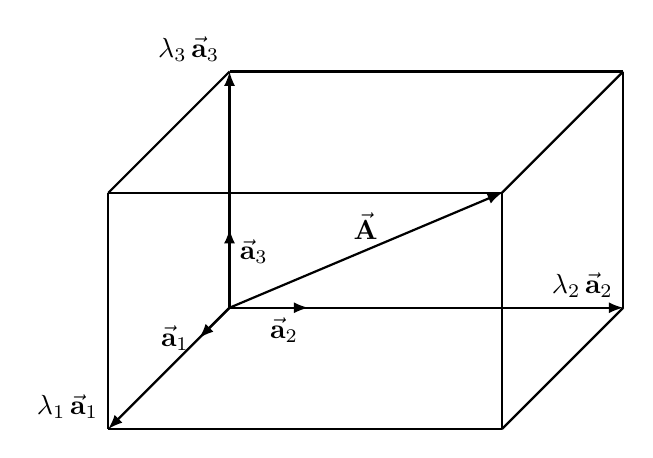
\begin{tikzpicture}
    %\tikzstyle{every node}=[font=\small]

    %vectores unitarios
    \draw[thick,-latex] (0, 0, 0) -- (0, 0, 1) node[anchor= east] {$\va{a}_{1}$};
    \draw[thick,-latex] (0, 0, 0) -- (1, 0, 0) node[anchor=north east] {$\va{a}_{2}$};
    \draw[thick,-latex] (0, 0, 0) -- (0, 1, 0) node[anchor=north west] {$\va{a}_{3}$};
   
    %vectores extendidos
    \draw[thick,-latex] (0, 0, 0) -- (0, 0, 4) node [above left, pos=1] {$\lambda_{1} \, \va{a}_{1}$};
    \draw[thick,-latex] (0, 0, 0) -- (5, 0, 0) node [above left, pos=1] {$\lambda_{2} \, \va{a}_{2}$};
    \draw[thick,-latex] (0, 0, 0) -- (0, 3, 0) node [above left, pos=1] {$\lambda_{3} \, \va{a}_{3}$};
    \draw[thick,-latex] (0, 0, 0) -- (5, 3, 4) node [midway, above] {$\va{A}$};
    
    \draw[thick] (0, 0, 4) -- (5, 0, 4);
    \draw[thick] (0, 3, 0) -- (5, 3, 0);
    \draw[thick] (5, 0, 0) -- (5, 0, 4);
   
    \draw[thick] (0, 3, 0) -- (0, 3, 4);
    \draw[thick] (0, 3, 4) -- (0, 0, 4);
    \draw[thick] (0, 3, 4) -- (5, 3, 4);
    \draw[thick] (5, 3, 4) -- (5, 3, 0);
    \draw[thick] (5, 3, 4) -- (5, 0, 4);
    \draw[thick] (5, 3, 0) -- (5, 0, 0);

    
\end{tikzpicture}
\end{document}